\mysection{Function arguments number statistics}
\label{args_stat}

I've always been interesting in what is average number of function arguments.

\myindex{UNIX!grep}
I've analyzed many Windows 7 32-bit DLLs \\
(crypt32.dll, mfc71.dll, msvcr100.dll, shell32.dll, 
user32.dll, d3d11.dll, mshtml.dll, msxml6.dll, sqlncli11.dll, wininet.dll, mfc120.dll, msvbvm60.dll, ole32.dll, themeui.dll, wmp.dll) 
(because they use \emph{stdcall} convention, and so it is easy to \emph{grep} disassembly output just by \INS{RETN X}).

\begin{itemize}
\item no arguments: $\approx 29\%$
\item 1 argument: $\approx 23\%$
\item 2 arguments: $\approx 20\%$
\item 3 arguments: $\approx 11\%$
\item 4 arguments: $\approx 7\%$
\item 5 arguments: $\approx 3\%$
\item 6 arguments: $\approx 2\%$
\item 7 arguments: $\approx 1\%$
\end{itemize}

\begin{figure}[H]
\centering
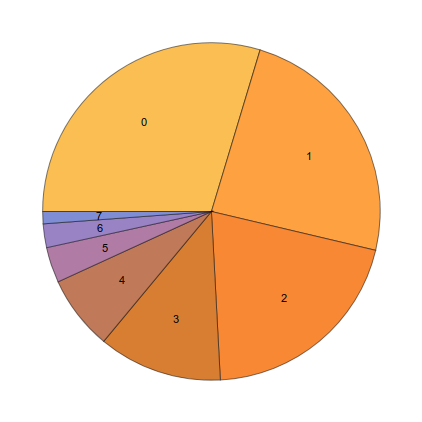
\includegraphics[width=0.5\textwidth]{other/args_stat.png}
\caption{Function arguments number statistics}
\end{figure}

This is heavily dependent on programming style and may be very different for other software products.

